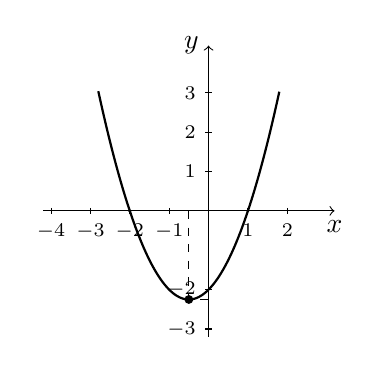
\begin{tikzpicture}[scale=0.5]
    \draw[->] (-4.2,0) -- (3.2,0) node[below] {$x$};
    \draw[->] (0,-3.2) -- (0,4.2) node[left] {$y$};
    \foreach \x in {-4,-3,-2,-1,1,2}
        \draw (\x,0.08) -- (\x,-0.08) node[below] {\scriptsize $\x$};
    \foreach \y in {-3,-2,1,2,3}
        \draw (0.08,\y) -- (-0.08,\y) node[left] {\scriptsize $\y$};
    \draw[smooth, samples=200, domain=-2.8:1.8, thick] plot (\x, {\x*\x+\x-2});
    \fill (-2,0) circle (1.2pt);
    \fill (1,0) circle (1.2pt);
    \fill (-0.5,-2.25) circle (3.2pt);
    \draw[dashed] (-0.5,0) -- (-0.5,-2.25);
    \draw[dashed] (0,-2.25) -- (-0.5,-2.25);
\end{tikzpicture}
